\documentclass[herrin-thesis.tex]{subfiles}
\begin{document}

\chapter{Neutrinos}
\label{ch:neutrinos}

\section{History}
Neutrino physics first arose in the study of beta decay. In the most basic form of beta decay, a neutron in a nucleus decays to a proton and emits an electron. Early nuclear physicists observed that unlike alpha particles and gamma rays, which are emitted in monoenergetic lines from nuclear processes, beta decay electrons are emitted with a continuous range of energies up to some maximum energy (known as the Q value). Rather than abandoning the principle of energy conservation, Wolfgang Pauli in 1930 proposed a massless particle that could carry away the ``missing energy'' in beta decays. In 1933, Enrico Fermi \cite{Fermi:1934bh} combined the idea with Werner Heisenberg's nucleon model to form a theory of beta decay. The proposed massless particle was eventually dubbed the ``neutrino''.

For several decades after Pauli proposed the neutrino, the only evidence for its existence was indirect. It was not until 1956 that Cowan and Reines \cite{Cowan:1956qf} observed the electron antineutrino by looking for the inverse beta decay reaction of antineutrinos from a nuclear reactor. In 1962, Lederman, Schwartz, and Steinberger \cite{Danby:1962ve} used a beam of pions decaying to muons to create a beam of neutrinos. These neutrinos interacted to form only muons and not electrons. This established the existence of the muon neutrino, distinct from the electron neutrino. These distinct types of neutrino with respect to the weak interaction are referred to as ``flavors''.

Beginning in the early 1970s, the Homestake experiment \cite{Cleveland:1998ly} observed a large deficit in the flux of electron neutrinos coming from the sun compared to the expected flux. Eventually, it was suggested that this ``solar neutrino problem'' was due to neutrinos oscillating between flavors in flight. The Super-Kamiokande experiment first observed evidence for neutrino oscillation in 1998 \cite{Fukuda:1998zr} by looking at neutrinos produced in the upper atmosphere. The solar neutrino problem was not definitively resolved until 2001 when the Sudbury Neutrino Observatory \cite{Ahmad:2001ys} simultaneously measured the flux of electron neutrinos and the total flux of all neutrinos from the sun. The total flux matched expectations, meaning that the missing electron neutrinos oscillated to other flavors in flight. For neutrinos to oscillate, they must have mass, and their mass eigenstates must be mixtures of the flavor eigenstates that participate in the weak interaction. Neutrino oscillations and neutrino masses have now become the subject of much research.

\section{The Nature of Neutrinos}
\subsection{Dirac Particles}
In the standard model of particle physics, neutrinos are massless and have left-handed chirality, forming a doublet with the left-handed charged leptons under the SU(2) symmetry of the weak force. The right-handed charged leptons form an SU(2) singlet, and there are no right-handed neutrinos. The mass of a charged lepton is generated by a Yukawa coupling between the left-handed lepton, the right-handed lepton, and the Higgs field. Since neutrinos have been observed to have mass, then, it seems natural to generate their mass in an analogous way. Masses due to this mechanism are known as Dirac masses. This would introduce right-handed neutrinos (and left-handed antineutrinos) that would not interact weakly. However, given the observed smallness of neutrino masses, this requires Yukawa couplings much, much smaller than those of charged leptons and quarks. Such small Yukawa couplings are difficult to explain.

\subsection{Majorana Particles}
Neutrinos do not carry charge, and so mass terms of the form
\begin{equation}
\mathcal{L}_{m}^{\nu} = -\frac{1}{2}\overline{\nu_{L}} m_{L L}^{\nu} \nu_{L}^{c} +h.c.
\label{eq:nu_majorana_lagrangian}
\end{equation}
can be added to the standard model Lagrangian. Such terms are not allowed for charged leptons, since they would violate electric charge conservation. No fundamental rule requires total lepton number conservation in the standard model, and so it is not troublesome that these terms violate it. Particles that have such mass terms satisfy the Majorana equation:
\begin{equation}
i\gamma^{\mu}\partial_{\mu}\psi - m \psi^{c} = 0
\end{equation}
The Majorana equation is similar to the Dirac equation, except that it includes the charge conjugate \(\psi^c\) of the spinor \(\psi\). Adding the supplemental condition that \(\psi^c = \psi\) results in a single neutral particle solution. This means Majorana particles can be described as their own antiparticles.

Mass terms like those in \cref{eq:nu_majorana_lagrangian} for left-handed neutrinos violate weak isospin symmetry, but can arise from other phenomena that conserve it. In 1979, S.~Weinberg \cite{Weinberg:1979qa} proposed a dimension 5 operator coupling the neutrino fields to the standard model Higgs field. However, such a term is not renormalizable and would have to reflect new physics at a mass scale much larger than the weak scale. Introducing massive right-handed Majorana neutrinos provides one possible mechanism. With right-handed neutrinos, the most general way to write the mass terms for one generation is
\begin{equation}
\mathcal{L}_{m}^{\nu} = -\frac{1}{2}
\begin{pmatrix}
	\overline{\nu_{L}} 	&	\overline{\nu_{R}^{c}}
\end{pmatrix}
\begin{pmatrix}
	m_{L L} 		&	m_{L R}			\\
	m_{L R}		&	M_{R R}
\end{pmatrix}
\begin{pmatrix}
	\nu_{L}^{c}	\\
	\nu_{R}
\end{pmatrix} + h.c.
\label{eq:nu_mass_matrix}
\end{equation}
where \(m_{L R}\) is a Dirac mass and \(m_{L L}\) and \(M_{R R}\) are Majorana masses. Diagonalizing this yields two mass eigenstates:
\begin{equation}
m_{\pm} = \frac{1}{2}\left | (M_{R R} + m_{L L}) \pm \sqrt{\left(M_{R R} - m_{L L}\right)^2 + 4 m_{L R}^2}\right |
\label{eq:nu_diagonalized_masses}
\end{equation}
The case in which \(m_{L L} = 0\) (which it must be to conserve weak isospin symmetry) and \(M_{R R}\gg m_{L R}\) is known as a type I seesaw mechanism. In this case, \(m_{-} \approx m_{L R}^2/M_{R R}\) and \(m_{+} \approx M_{R R}\). Suppose \(m_{L R}\) is on the order of quark or charged lepton masses. If \(M_{R R}\) is much greater than the electroweak scale, then the light neutrino masses (\(m_{-}\)) take on small values. The light neutrinos are a mixture of left and right-handed neutrinos, but the right-handed amplitude is suppressed by \(m_{L R}/M_{R R}\) and so is negligible.

\subsection{Majorons}
\label{sec:nu_majoron_theory}
Instead of right-handed neutrinos, suppose there is instead a new set of Higgs-like particles \(\phi^0\), \(\phi^{-}\) and \(\phi^{--}\) that forms a complex triplet under the weak interaction. If, analogously to the standard Higgs, \(\phi^0\) acquires a vacuum expectation value \(\langle\phi^0\rangle\) through the spontaneous breaking of lepton number symmetry, then interactions with the neutrino fields can give Majorana neutrino mass terms with \(m_{L L} = \lambda \langle\phi^0\rangle\), where \(\lambda\) is a Yukawa coupling.

If the vacuum expectation value \(\langle\phi^0\rangle\) were small, this would lead to small neutrino masses. Furthermore, analogously to the standard Higgs mechanism, the spontaneous symmetry breaking would lead to a Goldstone boson known as the Majoron. This theory, due to Gelmini and Roncadelli \cite{Gelmini:1981uq} and Georgi et al. \cite{Georgi:1981kx} is disfavored due to precise measurements of the width of the \(Z^{0}\) decay to invisible channels.

Another theory, due to Chikashige et al. \cite{Chikashige:1981vn} introduces a Higgs-like singlet that acquires a vacuum expectation value and gives a Majorana mass to right-handed neutrinos. The light neutrinos acquire mass through a seesaw mechanism as above, but the symmetry breaking again creates a Majoron. This theory contributes to the \(Z^{0}\) width at a level less than the current uncertainty on the measurement, and so is not ruled out. Other models \cite{Berezhiani199299,Bamert:1995fk} have been proposed that are consistent with LEP data on the \(Z^{0}\) width.

\section{Neutrino Mixing and Oscillation}
Neutrinos are observed to oscillate, which implies that the mass eigenstates that propagate are different from the flavor eigenstates that participate in the weak interaction. Neutrino mixing is described by the unitary Pontecorvo-Maki-Nakagawa-Sakata (PMNS) matrix \(U\). In the case of three mass eigenstates and 3 flavor eigenstates, \(U\) can be parameterized by three Euler rotation angles, one Dirac CP violation phase, and two Majorana CP violation phases (if neutrinos are Majorana particles):
\begin{align}
U =&\begin{pmatrix}
	U_{e1}	&	U_{e2}	& 	U_{e3}	\\
	U_{\mu1}	&	U_{\mu2}	& 	U_{\mu3}	\\
	U_{\tau1}	&	U_{\tau2}	& 	U_{\tau3}	\\
	\end{pmatrix}\\
%     =&\begin{pmatrix}
%	1	&	0		&	0		\\
%	0	&	c_{23}	&	s_{23}	\\
%	0	&	-s_{23}	&	c_{23}	\\
%	\end{pmatrix}
%	\begin{pmatrix}
%	c_{13}			&	0	&	s_{13}e^{-i\delta}	\\
%	0				&	1	&	0				\\
%	-s_{13}e^{i\delta}	&	0	&	c_{13}			\\
%	\end{pmatrix}
%	\begin{pmatrix}
%	c_{12}	&	s_{12}	&	0	\\
%	-s_{12}	&	c_{12}	&	0	\\
%	0		&	0		&	1	\\
%	\end{pmatrix}
	=&\begin{pmatrix}
	c_{12}c_{13}							&	s_{12}c_{13}							&	s_{13}e^{-i\delta}	\\
	-s_{12}c_{23}-c_{12}s_{23}s_{13}e^{i\delta}	&	c_{12}c_{23}-s_{12}s_{23}s_{13}e^{i\delta}	&	s_{23}c_{13}		\\
	s_{12}s_{23}-c_{12}c_{23}s_{13}e^{i\delta}	&	-c_{12}s_{23}-s_{12}c_{23}s_{13}e^{i\delta}	&	c_{23}c_{13}
	\end{pmatrix}
	\begin{pmatrix}
	1	&	0					&	0	\\
	0	&	e^{\frac{i\alpha_{21}}{2}}	&	0	\\
	0	&	0					&	e^{\frac{i\alpha_{31}}{2}}
	\end{pmatrix}\nonumber
\label{eq:nu_pmns_matrix}
\end{align}
where the \(s_{ij}\) denote \(\sin\theta_{ij}\) and \(c_{ij}\) denote \(\cos\theta_{ij}\). \(\delta\) is the Dirac CP violation phase, and \(\alpha_{21}\) and \(\alpha_{31}\) are the Majorana CP violation phases.

 A flavor eigenstate, such as a neutrino produced by the decay of a lepton, is a superposition of mass eigenstates:
 \begin{equation}
 \Ket{\nu_{\ell}} = \sum_{i}U_{\ell i}^{*} \Ket{\nu_i}
 \label{eq:nu_superposition}
 \end{equation}
 This mixing is illustrated in \cref{fig:nu_mixing}.
 
 The time evolution of a mass eigenstate is simply
 \begin{equation}
 \Ket{\nu_{i}(t)} = e^{-i(E_i t - \vec{p}_i\cdot\vec{x})}\Ket{\nu_i(0)}
 \label{eq:nu_time_evolution}
 \end{equation}

Neutrinos have such small masses that they are always observed in a ultrarelativistic state, in which \(t\approx L\) and \(p\approx E\), where \(E\) is the total energy of the neutrino. In this limit, the phase in the exponent for \cref{eq:nu_time_evolution} becomes \(m_i^2 L/(2E)\). Combining this and \cref{eq:nu_superposition}, the probability for a neutrino with flavor \(\alpha\) and energy \(E\) to oscillate to a neutrino with flavor \(\beta\) after traveling distance \(L\) is
\begin{align}
P_{\alpha\rightarrow\beta}	&=& \left | \Braket{\nu_\beta | \nu_\alpha(L)} \right |^2	& =& \delta_{\alpha\beta}	& - 4\sum_{i>j}\text{Re}\left(U_{\alpha i}^{*}U_{\beta i}U_{\alpha j}U_{\beta j}^{*}\right)\sin^2\left(\frac{\Delta m_{ij}^2 L}{4 E}\right)\nonumber\\
						&  &											&   &					& +2\sum_{i>j}\text{Im}\left(U_{\alpha i}^{*}U_{\beta i}U_{\alpha j}U_{\beta j}^{*}\right)\sin^2\left(\frac{\Delta m_{ij}^2 L}{2 E}\right)
\label{eq:nu_oscillation_prob}
\end{align}

Thus, the probability depends only on the parameters in the mixing matrix \(U\), the difference between the squares of the masses \(\Delta m_{ij}^2\), and the ratio of distance travelled to neutrino energy \(L/E\). If there is no CP violation, \(U\) is real and the second sum is zero. Since the Majorana phases only enter \(U\) as a diagonal factor, they do not affect the oscillation probability, and thus oscillation experiments cannot determine the Majorana nature of the neutrino.

\section{Measuring Neutrino Masses}

\begin{figure}[htp]
	\centering
	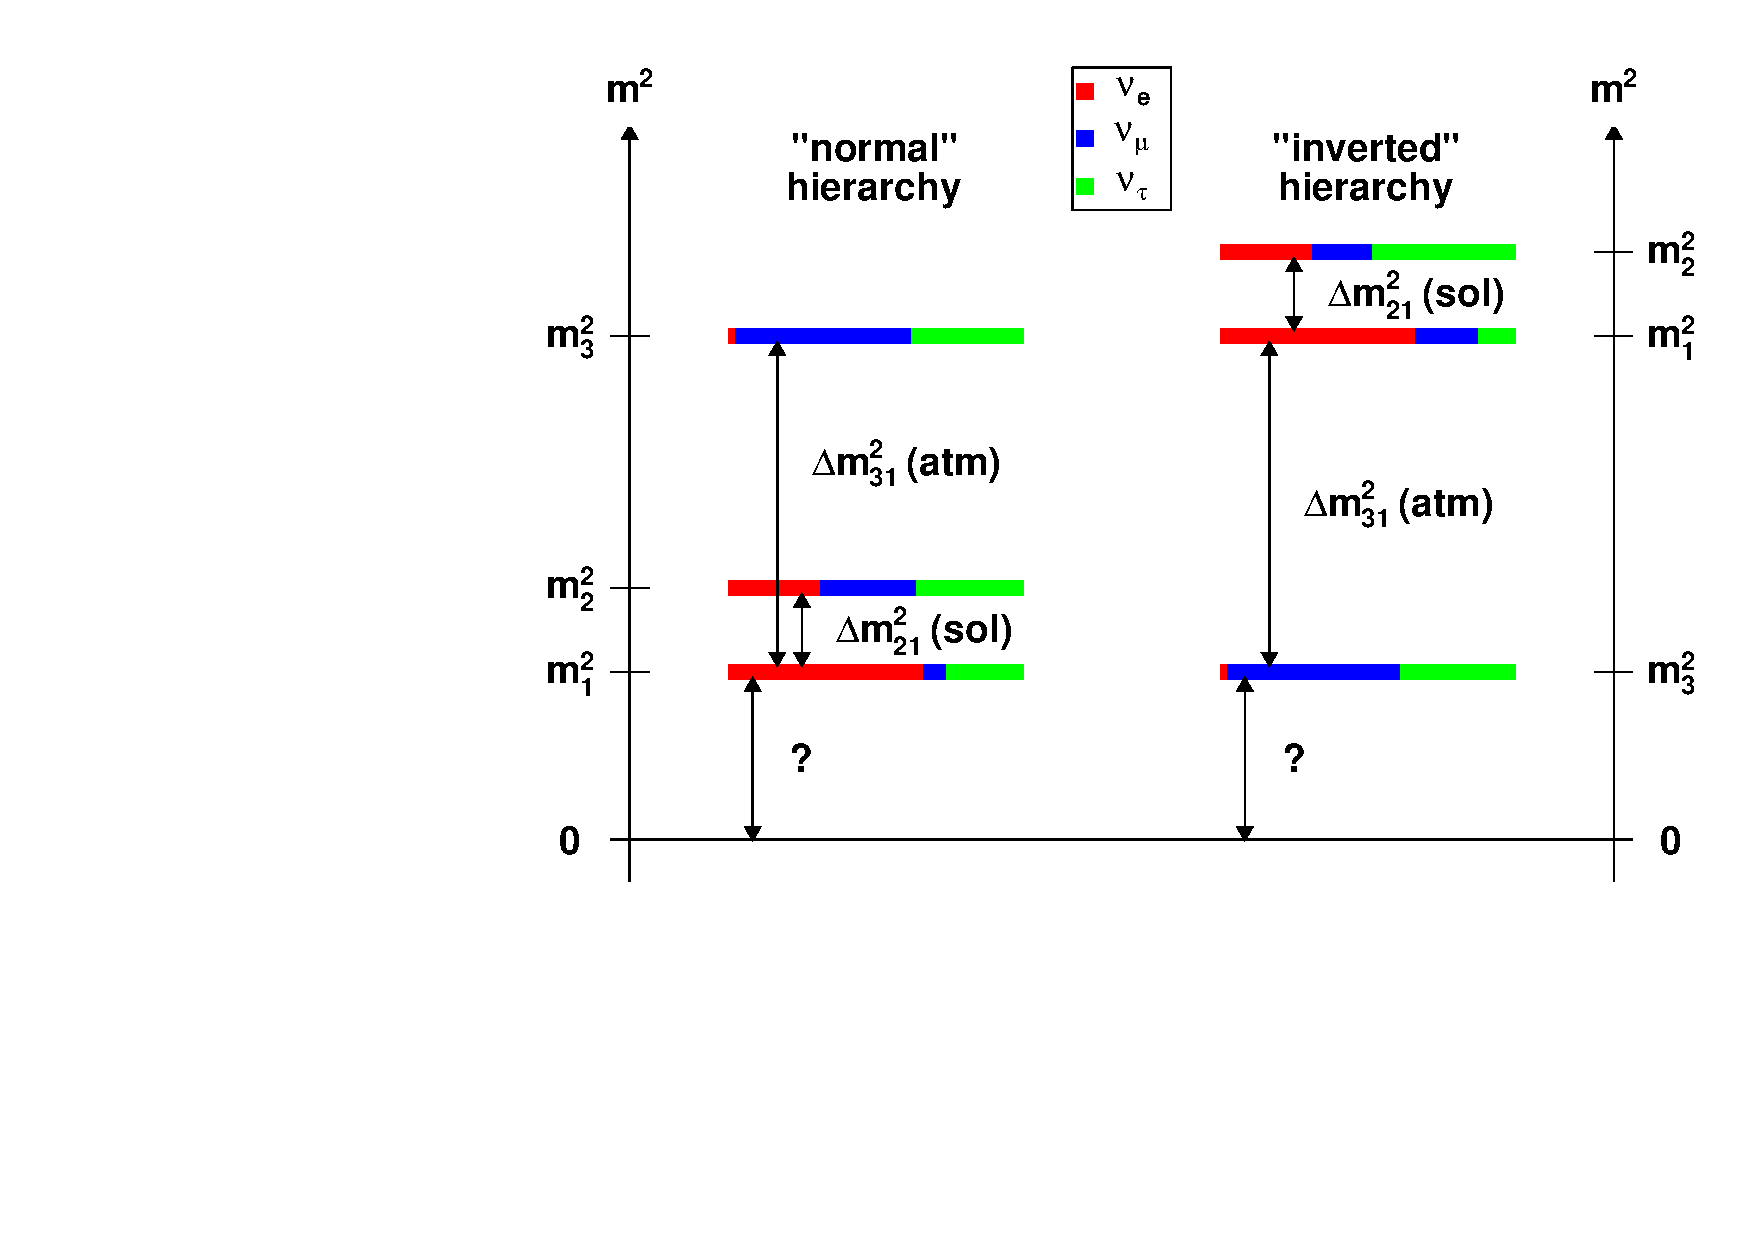
\includegraphics[width=0.6\textwidth]{./plots/nu_mixing.pdf}
	\caption[Neutrino mixing and mass hierarchy]{The neutrino mass eigenstates (represented by the horizontal bands) are each a mixture of the flavor eigenstates (represented by the different colors). The mixing angles in the PMNS matrix provide the flavor compositions of each mass state. The splittings between the squares of the masses of the mass eigenstates are known (but not shown to scale), though the sign of \(\Delta m_{31}^2\) remains unknown, allowing for the possibility of an ``inverted'' mass hierarchy. The absolute scale of the neutrino masses is also unknown.}
	\label{fig:nu_mixing}
\end{figure}

From oscillation experiments, it is known that the mass-squared splittings in \cref{eq:nu_oscillation_prob} are nonzero. The mass state \(\nu_1\) has been defined as the one with the largest \(\nu_e\) component. Under this convention, the sign of \(\Delta m_{21}^2\) is known from the effect of solar matter on neutrinos emitted by the sun (known as the MSW effect), while only the magnitude of \(\Delta m_{31}^2\) is known. The mass splittings provide lower bounds on the masses of two mass eigenstates. This does not determine the absolute mass scale, however, and the lightest eigenstate may have zero mass. Since the sign of \(\Delta m_{31}^2\) remains unknown, it is unknown which mass eigenstate is the lightest. \Cref{fig:nu_mixing} summarizes the situation. Other experiments, described below, may be able to measure the absolute mass scale and possibly determine the hierarchy of the mass eigenstates. However, to date, such experiments have only provided upper bounds on the mass.

\subsection{Beta Decay Endpoint}
\begin{figure}[htp]
	\centering
	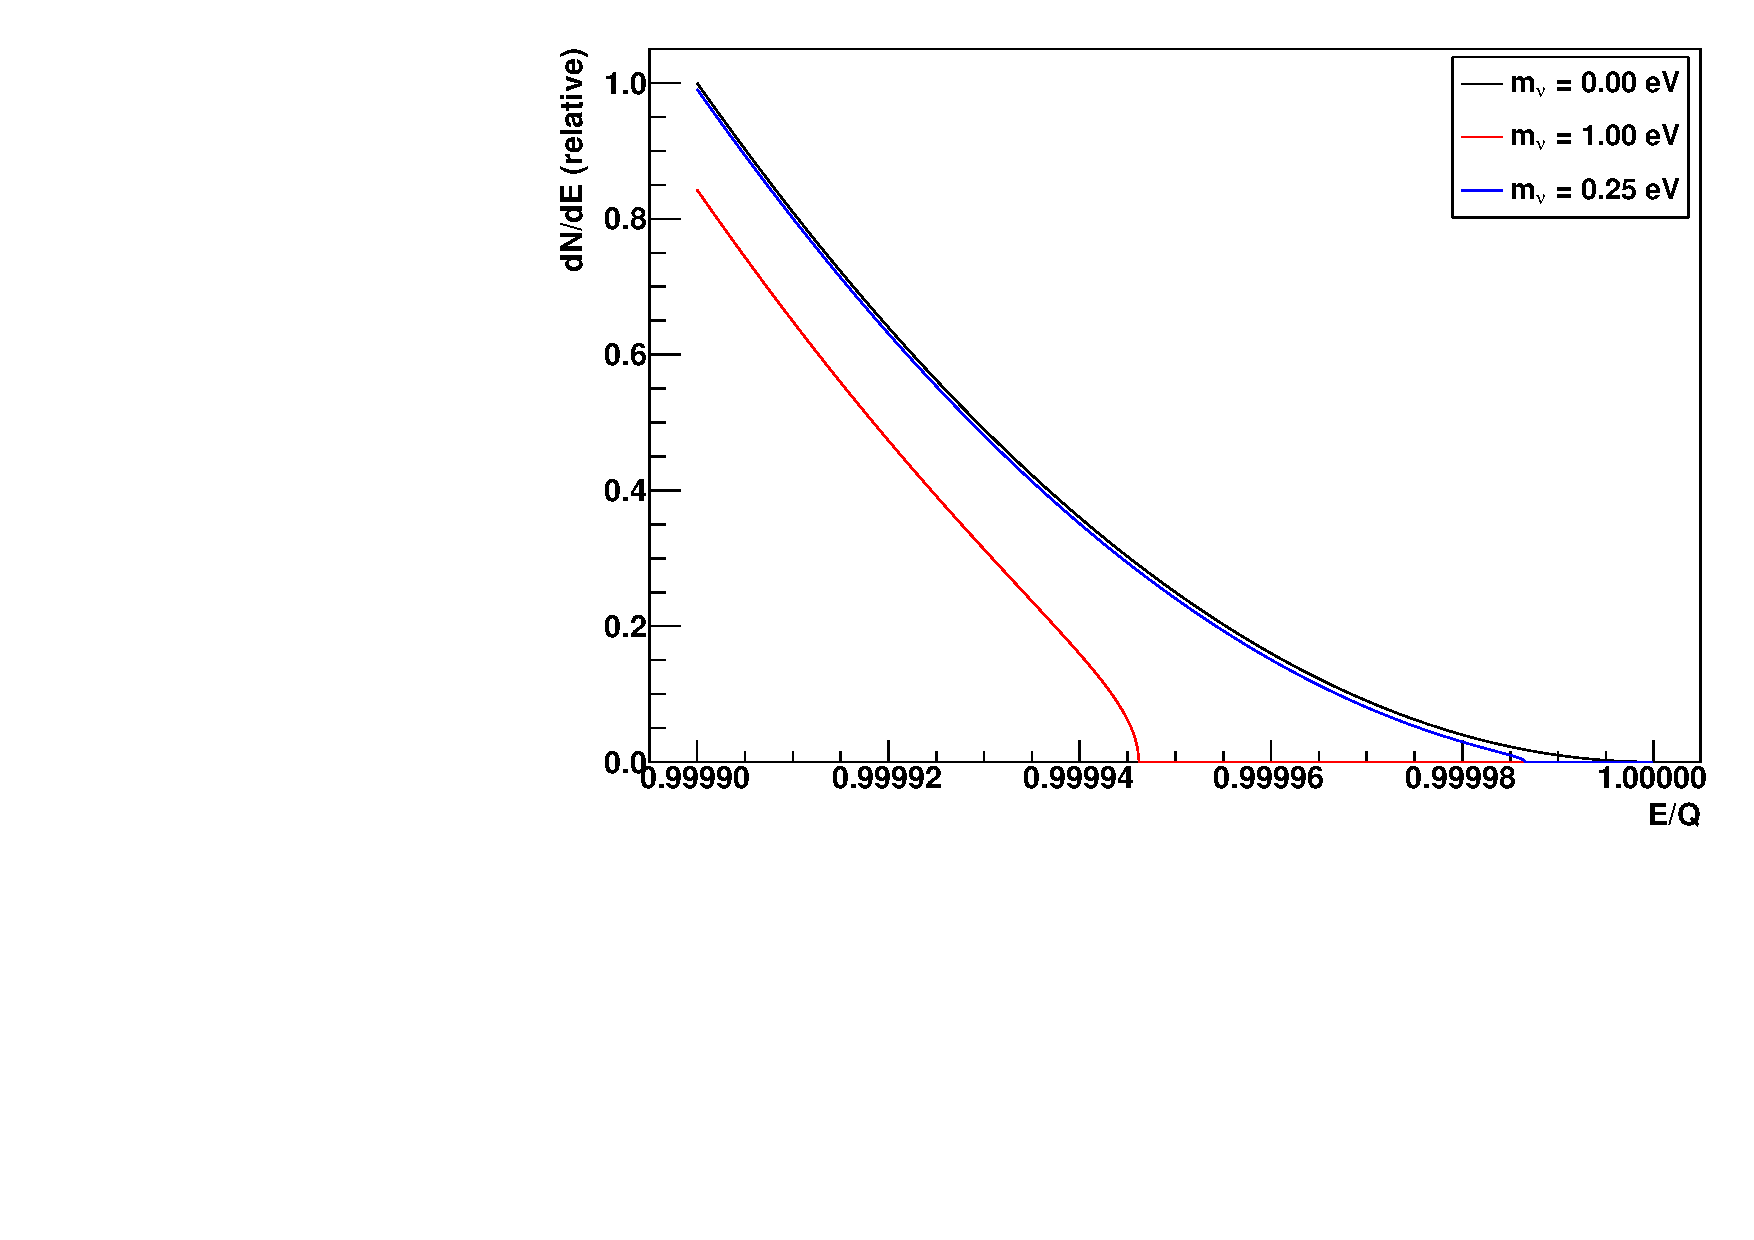
\includegraphics[width=0.6\textwidth]{./plots/nu_beta_endpt.pdf}
	\caption[Beta decay spectrum endpoint for massive neutrinos]{The endpoint of the electron energy spectrum for beta decay for several neutrino masses. Experiments like Mainz \cite{Kraus:2005nx}, Troitsk \cite{Aseev:2011dq}, and KATRIN \cite{Osipowicz:2001oq} aim to measure the neutrino mass by looking for the slight distortion of the spectrum close to the Q value of the decay due to the neutrino mass.}
	\label{fig:nu_beta_endpt}
\end{figure}

When a nucleus beta decays, it emits an electron antineutrino, which carries away some energy from the decay. However, this amount may be very small, and so in rare cases, the electron may carry away nearly all of the energy. A neutrino with nonzero rest mass will always take some energy to create, however, limiting the maximum energy of the electron and distorting the spectrum near the upper end of its range. This is illustrated in \cref{fig:nu_beta_endpt}.

An experiment looking for this distortion in the beta decay spectrum will measure the effective mass squared of the electron neutrino:
\begin{equation}
m^2\left(\nu_e\right) = \sum_j \left | U_{e j} \right |^2 m^2\left(\nu_j\right)
\label{eq:nu_beta_endpt_mass}
\end{equation}
The best limits come from the Mainz and Troitsk experiments, which examined the spectrum of tritium. Mainz measured \(m(\nu_e) \leq 2.3 \text{ eV}/\text{c}^{2}\) \cite{Kraus:2005nx}, while Troitsk measured \(m(\nu_e) \leq 2.05 \text{ eV}/\text{c}^{2}\) \cite{Aseev:2011dq}, both at the 95\% confidence level. The KATRIN experiment, which will begin operation soon and also examine the spectrum for tritium, hopes to be sensitive to masses greater than \(0.2\text{ eV}/\text{c}^2\) \cite{Osipowicz:2001oq}.

\subsection{Cosmology}
Due to their small masses and large velocities, neutrinos in the early universe did not clump together as much as other matter. The distribution of matter in the universe, then, is sensitive to the mass ratio of neutrinos to other matter. Cosmological surveys of structure and anisotropy can potentially measure \(\sum m_{\nu}\). Cosmic microwave background data from the Planck satellite provide the best limit to date. The Planck data yield \(\sum m_{\nu} < (0.23 - 1.08) \text{ eV}/\text{c}^2\). The spread is due to the choice of model and which datasets are combined in the analysis \cite{Ade:2013kl}. Further data from other surveys may push the sensitivity down to the \si{\eV} scale \cite{Abazajian:2011dt}.

\subsection{Double Beta Decay}
\label{sec:nu_doublebetadecay}

\subsubsection{Two-Neutrino-Emitting Double Beta Decay}

\begin{figure}[htp]
	\centering
	\includegraphics[width=0.48\textwidth]{./feynman_diagrams/twonubetabeta.pdf}
	\caption[\(2\nu\beta\beta\) decay]{The standard-model-allowed mode of two-neutrino-emitting double beta decay (\twonu{}).}
	\label{fig:nu_diagram_2nubb}
\end{figure}

Standard double beta decay (\twonu{}) is a standard model process in which two neutrons simultaneously decay to two protons, emitting two electrons and two antineutrinos. \Cref{fig:nu_diagram_2nubb} illustrates this process. It has been observed in a number of isotopes with half lives between \SI{7.1d18}{\year} for \isotope{100}{Mo} \cite{Arnold:2005hc} and \SI{2.2d21}{\year} for \xenon{136} \cite{Auger:2012ar}. The rate goes like:
\begin{equation}
\left [ T^{2\nu}_{1/2} \right ]^{-1} = G^{2\nu}\left(E, Z\right)\left| \mathcal{M}^{2\nu}\right |^2
\label{eq:nu_twonu_rate}
\end{equation}
where \(G(E,Z)\) is a known phase space factor and \(\mathcal{M}\) is the nuclear matrix element, which can be calculated using various nuclear structure models.

Any experiment looking for more exotic forms of double beta decay should also observe this standard mode. Studying the two-neutrino-emitting mode can constrain it as a background to these searches. Moreover, measuring the rate in turn measures the nuclear matrix element. For more exotic modes, models must be used to predict the nuclear matrix elements in order to translate the rates (or limits on the rates) into statements about neutrinos. These models can be evaluated by comparing their predictions to the measurement of the \twonu{} matrix element.

\subsubsection{Neutrinoless Double Beta Decay}

\begin{figure}[htp]
         \begin{subfigure}[b]{0.48\textwidth}
		\centering
		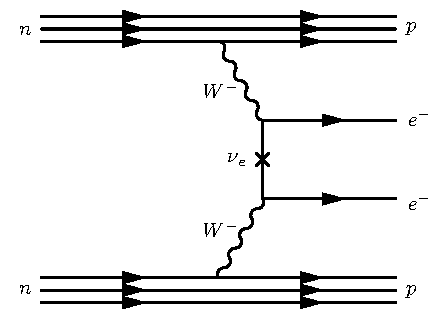
\includegraphics[width=\textwidth]{./feynman_diagrams/zeronubetabeta.pdf}
		\caption[\zeronu{} decay]{The simplest mode of neutrinoless double beta decay (\zeronu{}).}
		\label{fig:nu_diagram_0nubb}
	\end{subfigure}\hfill%
         \begin{subfigure}[b]{0.48\textwidth}
		\centering
		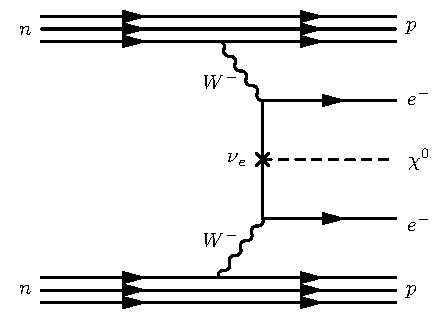
\includegraphics[width=\textwidth]{./feynman_diagrams/zeronubetabetamajoron.pdf}
		\caption[\zeronuX{} decay]{One neutrinoless mode of double beta decay with Majoron emission (\zeronuX{}).}
		\label{fig:nu_diagram_0nubbX}
	\end{subfigure}
	\caption[Neutrinoless double beta decay modes]{Neutrinoless double beta decay modes}
	\label{fig:nu_diagrams}
\end{figure}

\begin{figure}[htp]
         \begin{subfigure}[b]{0.48\textwidth}
		\centering
		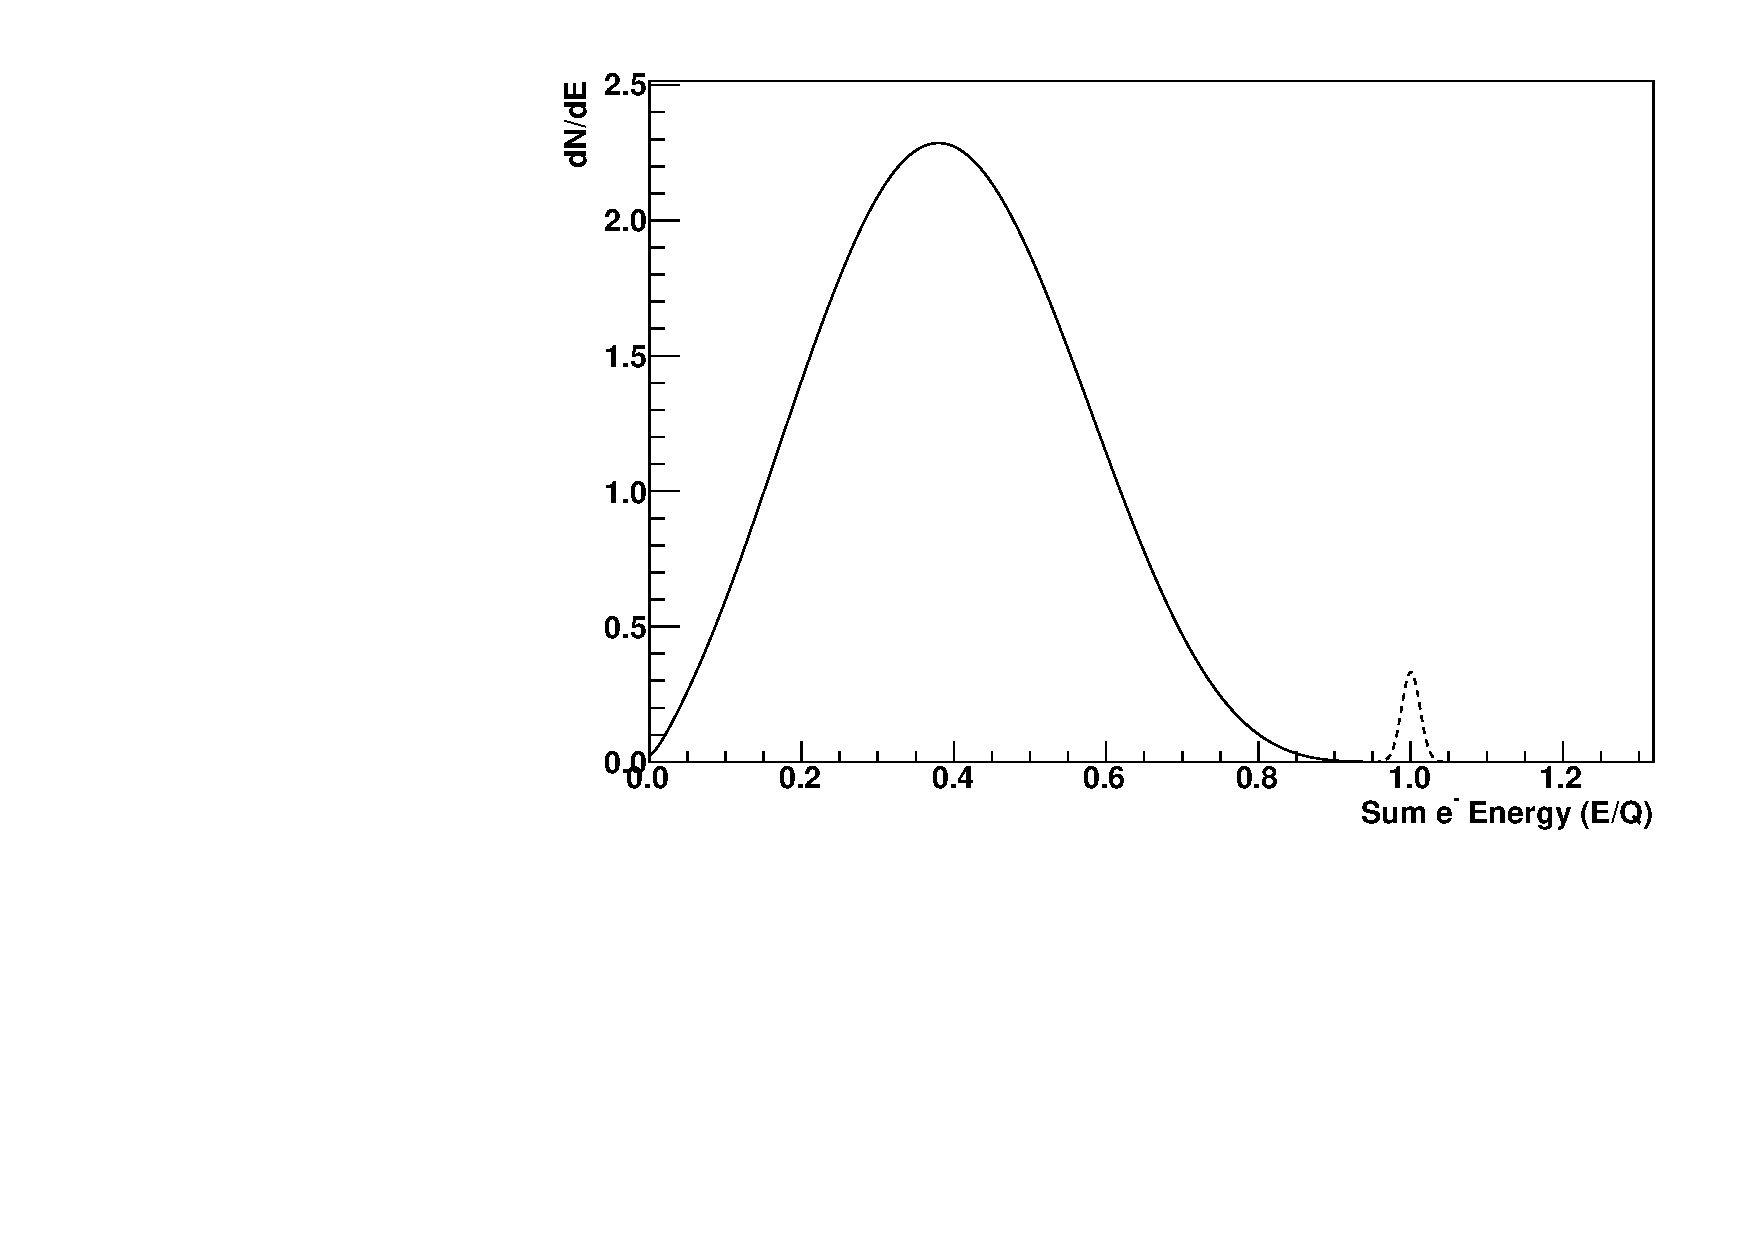
\includegraphics[width=\textwidth]{./plots/nu_comp_2nu_0nu_1e2.pdf}
	\end{subfigure}\hfill%
         \begin{subfigure}[b]{0.48\textwidth}
		\centering
		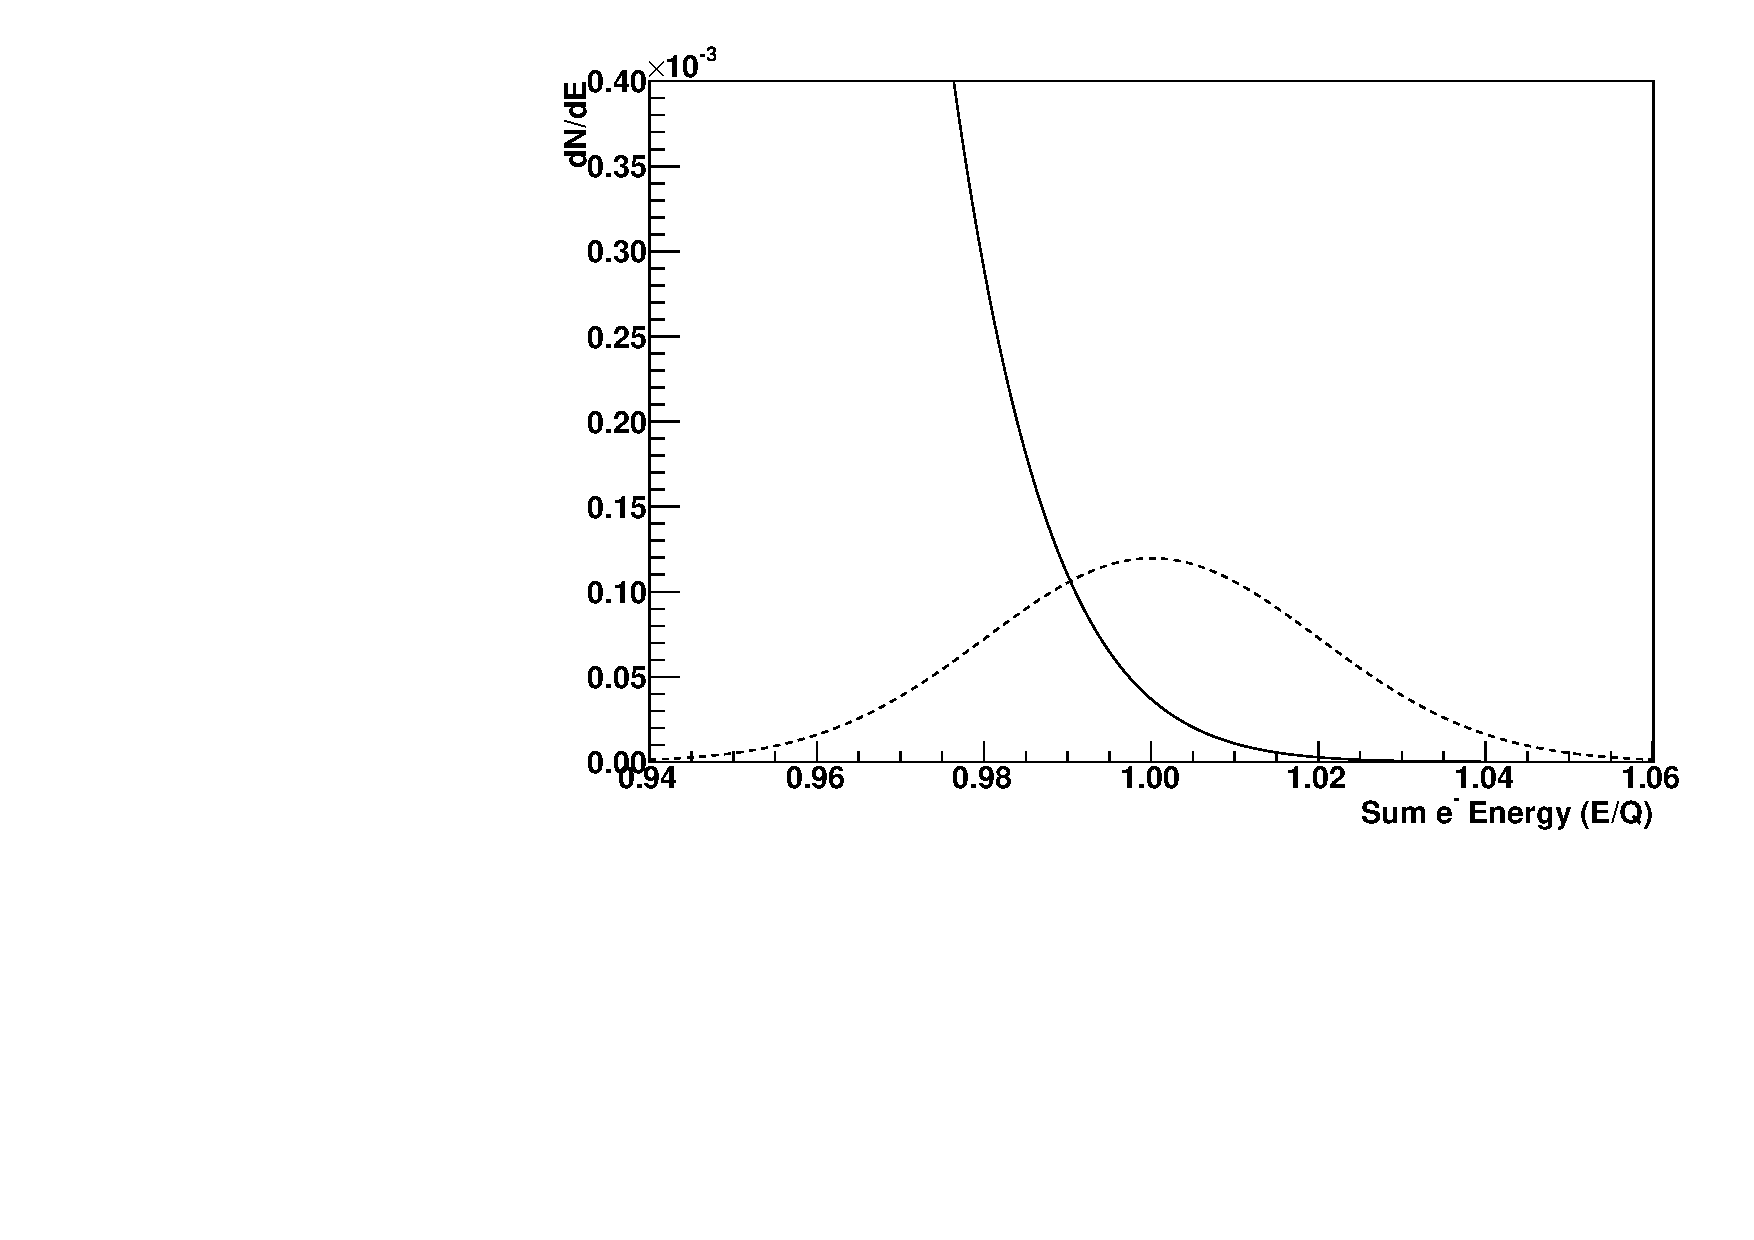
\includegraphics[width=\textwidth]{./plots/nu_comp_2nu_0nu_1e6.pdf}
	\end{subfigure}
	\caption[Comparison of \twonu{} and \zeronu{} energy spectra]{The electrons emitted in two-neutrino-emitting double beta decay have a continuous sum energy spectrum (solid line), while the energies of the electrons emitted in neutrinoless double beta decay sum to the Q value (dashed line). Here the spectra have been smeared with a 2\% \(\sigma/E\) energy resolution. On the left (right), the rate of \zeronu{} is 100 (\(1\times10^{6}\)) times less than that of \twonu{}. If the rate of \zeronu{} is small compared to \twonu{}, good energy resolution is needed to distinguish the two modes.}
	\label{fig:nu_comp_2nu_0nu}
\end{figure}

\begin{table}[tbp]
\centering
\caption[Current limits on \zeronu{}]{Results of searches for neutrinoless double beta decay. Effective masses are as reported by the experiments, and no attempt has been made to standardize the nuclear matrix element calculations used. Where a range has been reported, it is due to variation between different nuclear matrix element calculations.}
\label{tab:nu_zeronu_limits}
\begin{tabular}{c c c c}\toprule
	isotope			&	half-life (\(\times10^{22}\) \si{\year})	&	\(\left|\langle m_{\nu}\rangle\right |\) (\si{\eV})	&	experiment	\\\midrule
	\isotope{48}{Ca}	&	\(>5.8\)						&	\(< (3.5-22)\)								& 	\ce{CaF2(Eu)} scintillators \cite{Umehara:2008ij}\\
	\isotope{76}{Ge}	&	\(>1900\)						&	\(< 0.35\)									&	Heidelberg-Moscow \cite{Klapdor-Kleingrothaus:2001bs}\\
	\isotope{76}{Ge}	&	\(2230^{+440}_{-310}\)			&	\(0.32\pm0.03\)								&	Subset of H-M \cite{KlapdorKleingrothaus:2006ff}\\
	\isotope{82}{Se}	&	\(>36\)						&	\(< (0.89 - 2.43)\)							&	NEMO-3 \cite{Barabash:2011fv}\\
	\isotope{96}{Zr}		&	\(>0.92\)						&	\(< (7.2 - 19.5)\)								&	NEMO-3 \cite{Barabash:2011fv}\\
	\isotope{100}{Mo}	&	\(>110\)						&	\(< (0.45 - 0.93)\)							&	NEMO-3 \cite{Barabash:2011fv}\\
	\isotope{116}{Cd}	&	\(>17\)						&	\(< 1.7\)									&	Solotvina \cite{Danevich:2003dz}\\
	\isotope{130}{Te}	&	\(>280\)						&	\(< (0.30 - 0.71)\)							&	CUORICINO \cite{Andreotti:2011fu}\\
	\isotope{136}{Xe}	&	\(>1600\)						&	\(< (0.14 - 	0.38)\)							&	EXO-200 \cite{Auger:2012ar}\\
	\isotope{136}{Xe}	&	\(>1900\)						&	\(< (0.12 - 	0.25)\)							&	KamLAND-Zen \cite{Gando:2013fk}\\
	\isotope{150}{Nd}	&	\(>1.8\)						&	\( < (4.0 - 6.3)\)								&	NEMO-3 \cite{Barabash:2011fv}\\\bottomrule
\end{tabular}
\end{table}

If neutrinos are Majorana particles, then there is the potential to observe neutrinoless double beta decay (\zeronu{}). The simplest mechanism, shown in \cref{fig:nu_diagram_0nubb}, has a light Majorana neutrino being exchanged. In this process two electrons are emitted, but unlike \twonu{}, the electrons carry away the entire energy of the decay. Thus, this decay mode should be observable in a detector with good energy resolution. \Cref{fig:nu_comp_2nu_0nu} illustrates the difference in the sum electron spectrum for the two modes. If \zeronu{} does indeed proceed through light neutrino exchange, then the rate is given by
\begin{equation}
\left [ T^{0\nu}_{1/2} \right ]^{-1} = G^{0\nu}\left(E, Z\right)\left | \langle m_{\nu} \rangle \right |^2\left | \mathcal{M}^{0\nu}\right |^2
\label{eq:nu_zeronu_rate}
\end{equation}
where \(G^{0\nu}(E,Z)\) is a calculable phase-space factor, \( \mathcal{M}^{0\nu}\) is the nuclear matrix element, which can be estimated with models, and
\begin{equation}
\langle m_{\nu} \rangle = \sum_i U_{e i}^2 m_i
\label{eq:nu_meff_def}
\end{equation}
is known as the ``effective mass''. A number of experiments have attempted to look for neutrinoless double beta decay, but it has not yet been observed. A controversial claim by a subset of the Heidelberg-Moscow collaboration report discovery of \zeronu{} in \isotope{76}{Ge} \cite{KlapdorKleingrothaus:2006ff}, but this is in tension with results from \isotope{136}{Xe} experiments \cite{Auger:2012ar,Gando:2013fk}. \Cref{tab:nu_zeronu_limits} summarizes the present status of experiments.

\subsubsection{Majoron-Emitting Double Beta Decay}

\begin{figure}[htbp]
	\centering
	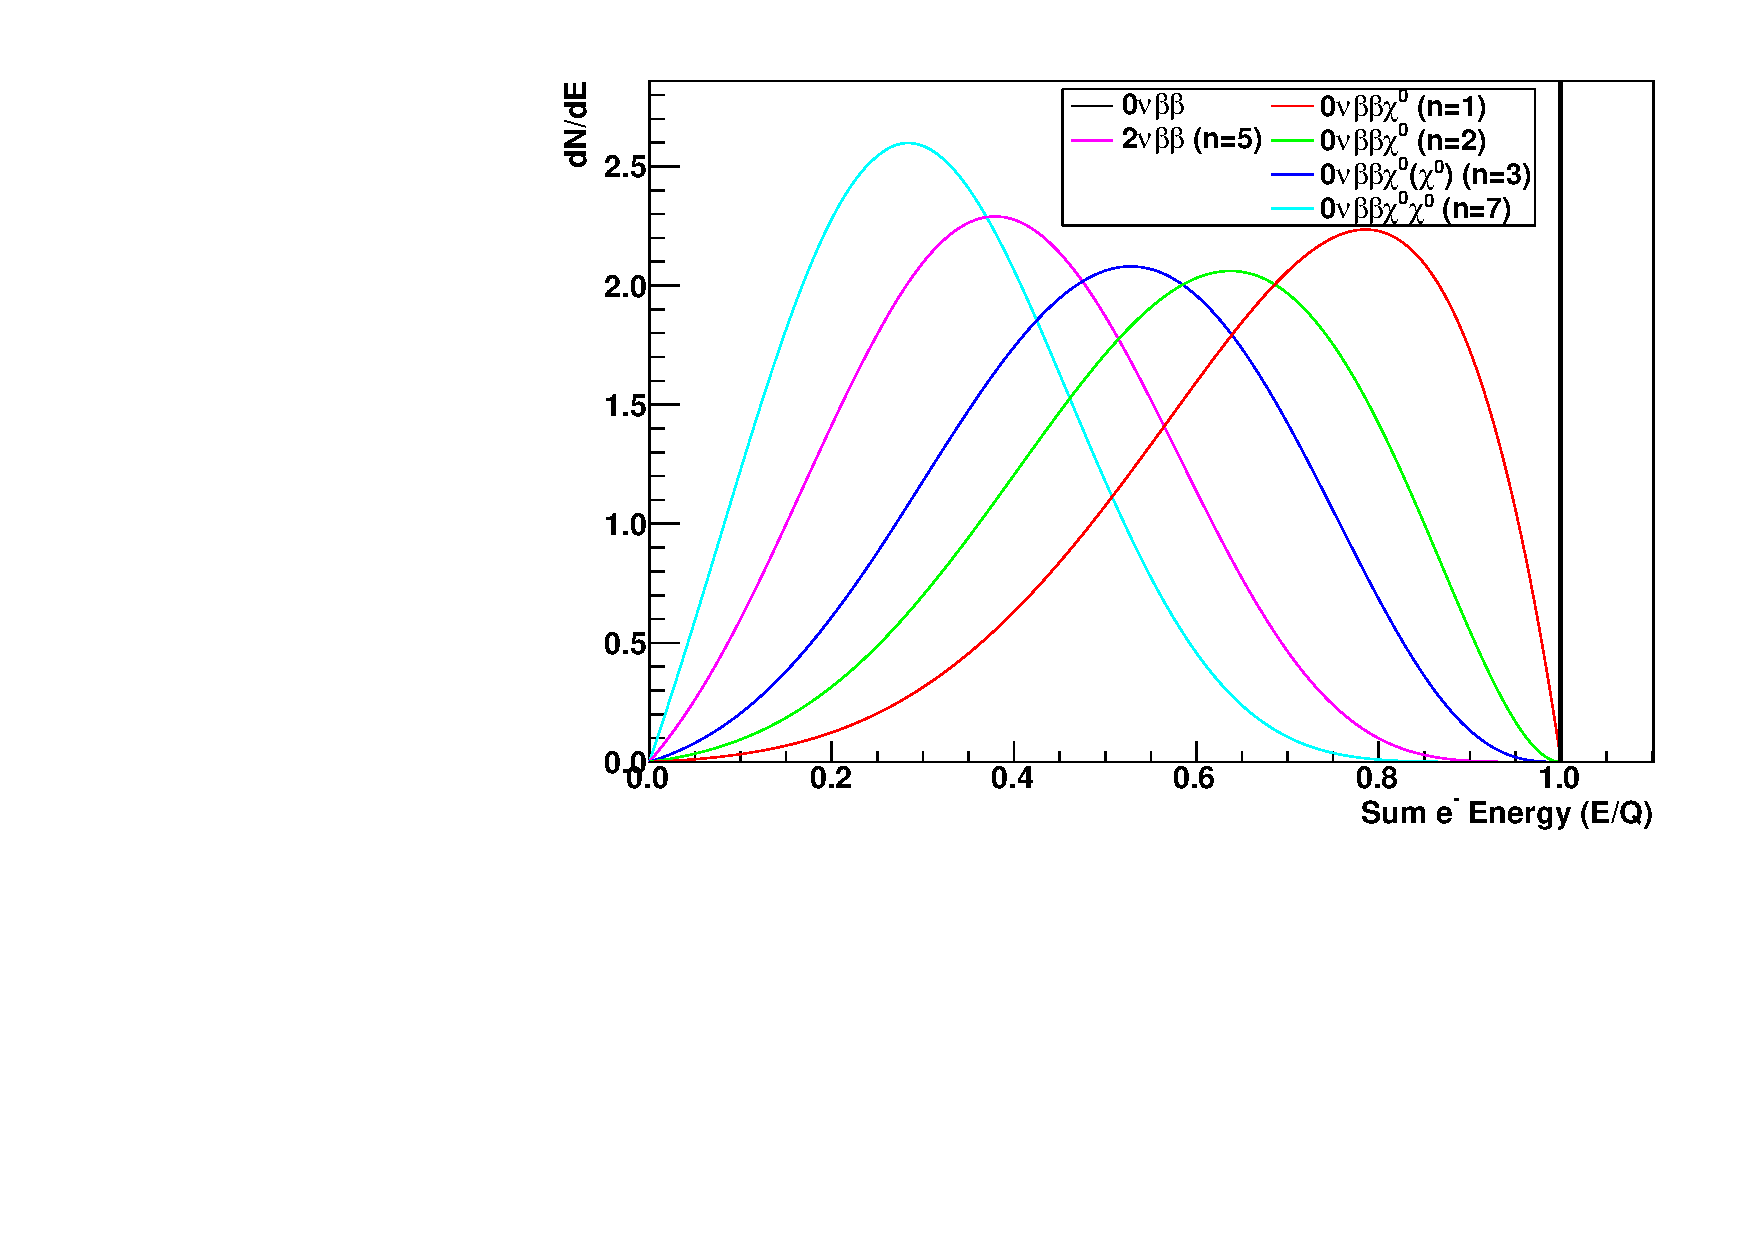
\includegraphics[width=0.6\textwidth]{./plots/nu_majoron_spectra}
	\caption[Energy spectra for Majoron-emitting double beta decay modes]{The sum electron energy spectra for different Majoron-emitting double beta decays. Decays with different spectral indices are clearly distinguishable. \twonu{} has a spectral index of 5 and is plotted for comparison. All spectra have been normalized.}
	\label{fig:nu_majoron_spectra}
\end{figure}

\begin{table}[hbp]
\centering
\caption[Current limits on \zeronuXpX{}]{Limits on the half-lives of Majoron-emitting double beta decay modes in \xenon{136} from the KamLAND-Zen experiment \cite{Gando:2012fk}.}
\label{tab:nu_majoron_limits}
\begin{tabular}{l c c}\toprule
	mode						&	spectral index \((n)\)		&	KamLAND-Zen 90\% C.L. \(T_{1/2}\) (yr)		\\\midrule
	\(0\nu\beta\beta\chi^{0}\)			&	1					&	\(>2.6\times10^{24}\)						\\
	\(0\nu\beta\beta\chi^{0}\)			&	2					&	\(>1.0\times10^{24}\)						\\
	\(0\nu\beta\beta\chi^{0}(\chi^{0})\)	&	3					&	\(>4.5\times10^{23}\)						\\
	\(0\nu\beta\beta\chi^{0}\chi^{0}\)	&	7					&	\(>1.1\times10^{22}\)						\\\bottomrule
\end{tabular}
\end{table}

There is also a possibility for double beta decay with the emission of one or more Majorons (\zeronuXpX{}), illustrated in \cref{fig:nu_diagram_0nubbX}. While the sum energy spectrum is not a sharp peak, it is still distinguishable from the two-neutrino-emitting mode by its shape, due to the different number of degrees of freedom for the invisible particle(s). As mentioned in \cref{sec:nu_majoron_theory}, a number of different theories predict Majoron emission. They differ in the nature of the Majoron (chiefly whether it carries lepton number, and whether it is a Goldstone boson) and in the number emitted. Regardless, the energy spectrum for the observable electrons is characterized by a single integer known as the ``spectral index''. \twonu{}, which similarly has invisible particles carrying away energy, has a spectral index of 5. Bamert et al. \cite{Bamert:1995fk} provide a thorough discussion of the different Majoron-emitting modes of double beta decay. \Cref{fig:nu_majoron_spectra} shows the spectra for proposed decay modes. The current best limits for Majoron-emitting modes in \xenon{136} come from the KamLAND-Zen collaboration \cite{Gando:2012fk} and are shown in \cref{tab:nu_majoron_limits}. The rate of a Majoron-emitting decay is
\begin{equation}
\left [ T^{\chi^0}_{1/2} \right ]^{-1} = G^{\chi^{0}}\left(E, Z\right)\left | \langle g_{e e} \rangle \right |^{2N}\left | \mathcal{M}^{\chi^{0}}\right |^2
\label{eq:nu_majoron_rate}
\end{equation}
where again \(G\) is a phase space factor and \(\mathcal{M}\) is a nuclear matrix element. \(N\) is the number of Majorons emitted. Theories predict \(N=1\) or \(N=2\). \(\langle g_{e e} \rangle\) is the effective coupling constant of the Majoron to the neutrino.

\subsubsection{Neutrinoless Double Beta Decay as a Black Box}

\begin{figure}[htp]
	\centering
	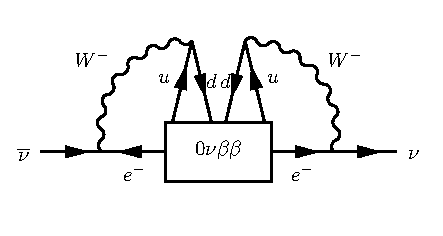
\includegraphics[width=0.6\textwidth]{./feynman_diagrams/zeronubetabeta_blackbox.pdf}
	\caption[Observation of \zeronu{} implies Majorana neutrinos]{Regardless of the mechanism by which \zeronu{} occurs, observation of neutrinoless double beta decay would imply Majorana neutrinos. This diagram corresponds to a Majorana mass term, treating \zeronu{} as a black box.}
	\label{fig:nu_blackbox}
\end{figure}

Even if neutrinoless double beta decay does not proceed through light neutrino exchange, any observation of neutrinoless double beta decay would imply that neutrinos are Majorana particles. This is illustrated in \cref{fig:nu_blackbox}. Treating \zeronu{} as a black box, a Majorana mass term can be constructed for neutrinos.

\subsection{Summary}

\begin{figure}[htp]
	\centering
	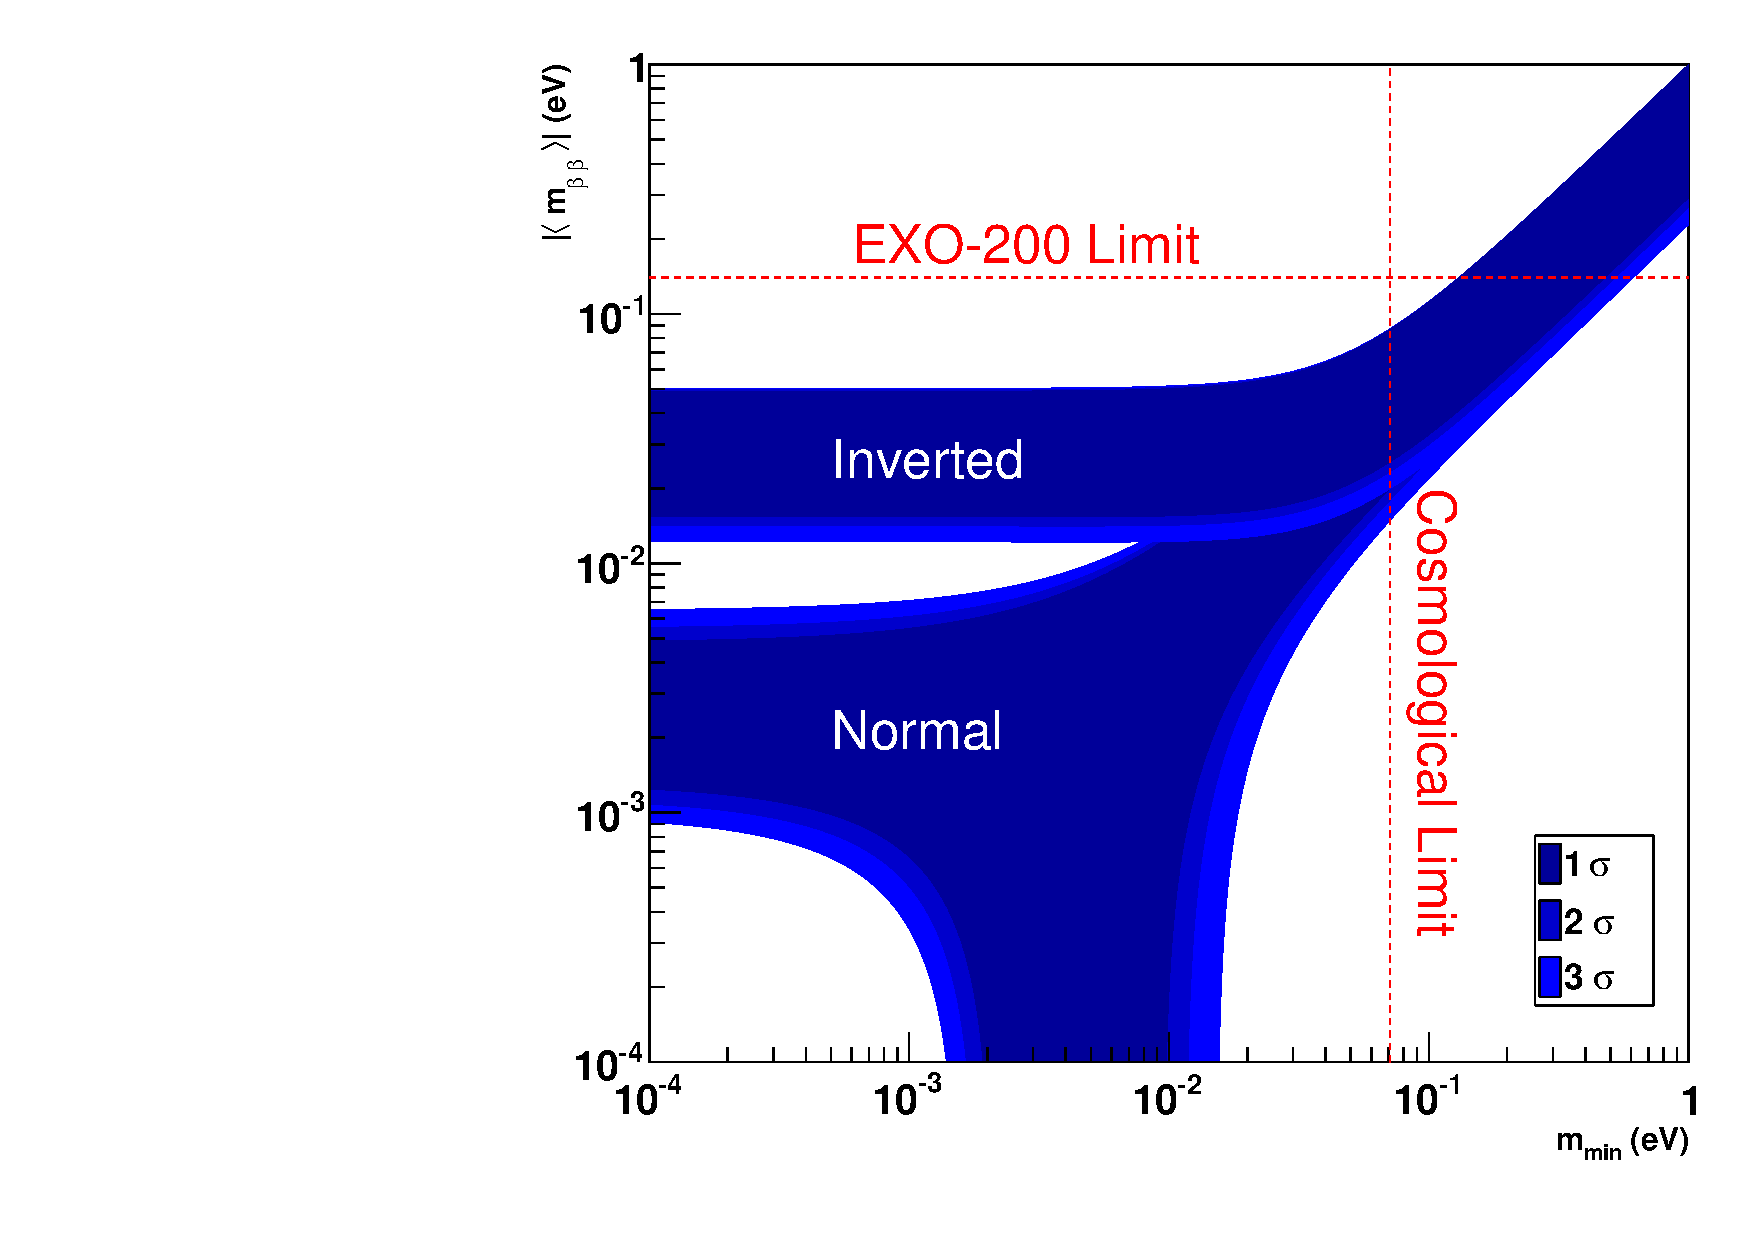
\includegraphics[width=0.6\textwidth]{./plots/nu_meff_v_mmin.pdf}
	\caption[Effective Majorana mass vs. smallest neutrino mass]{The allowed values for the effective Majorana mass as a function of the smallest neutrino mass for both the inverted and normal mass hierarchies. The widths of the bands depend on the Majorana phases. Uncertainties on the mixing angles and mass splittings widen these bands. The mixing angles, mass splittings, and uncertainties used are from a global fit by Forero et al. \cite{Forero:2012cr} The double beta decay limit comes from EXO-200 \cite{Auger:2012ar}, with the spread due to different nuclear models. The cosmological limit comes from the Planck 2013 data \cite{Ade:2013kl}, with the spread due to choice of model and which datasets are combined in the analysis. Constraints on the sum of the neutrino masses combined with the mass splittings yield an upper bound for the smallest neutrino mass.}
	\label{fig:nu_meff_v_mmin}
\end{figure}

The different experiments presented above are all complimentary. Double beta decay experiments, for example, may be able to determine the nature of neutrinos and, if they are Majorana particles, their mass scale. Oscillation experiments measure the mixing angles and mass splittings and should be able to determine the hierarchy, but as \cref{eq:nu_oscillation_prob} showed, they cannot determine the Majorana nature. \Cref{fig:nu_meff_v_mmin} shows one way in which these results can be combined. If, for example, the hierarchy is determined to be inverted, but double beta decay experiments rule out the corresponding mass range, then neutrinos are not Majorana particles. Meanwhile, tritium endpoint experiments and cosmology can potentially determine the mass scale, but cannot determine the Majorana nature of neutrinos.

\end{document}
